\documentclass[a4paper,10pt,ngerman]{scrartcl}
\usepackage{babel}
\usepackage[T1]{fontenc}
\usepackage[utf8x]{inputenc}
\usepackage[a4paper,margin=2.5cm,footskip=0.5cm]{geometry}

% Die nächsten drei Felder bitte anpassen:
\newcommand{\Aufgabe}{Aufgabe 2: Rechenrätsel} % Aufgabennummer und Aufgabennamen angeben
\newcommand{\TeilnahmeId}{63175}                  % Teilnahme-ID angeben
\newcommand{\Name}{Lars Noack}             % Name des Bearbeiter / der Bearbeiterin dieser Aufgabe angeben


% Kopf- und Fußzeilen
\usepackage{scrlayer-scrpage, lastpage}
\setkomafont{pageheadfoot}{\large\textrm}
\lohead{\Aufgabe}
\rohead{Teilnahme-ID: \TeilnahmeId}
\cfoot*{\thepage{}/\pageref{LastPage}}

% Position des Titels
\usepackage{titling}
\setlength{\droptitle}{-1.0cm}

% Für mathematische Befehle und Symbole
\usepackage{amsmath}
\usepackage{amssymb}

% Für Bilder
\usepackage{graphicx}

% Für Algorithmen
\usepackage{algpseudocode}

% Für Quelltext
\usepackage{listings}
\usepackage{color}
\definecolor{mygreen}{rgb}{0,0.6,0}
\definecolor{mygray}{rgb}{0.5,0.5,0.5}
\definecolor{mymauve}{rgb}{0.58,0,0.82}
\lstset{
  keywordstyle=\color{blue},commentstyle=\color{mygreen},
  stringstyle=\color{mymauve},rulecolor=\color{black},
  basicstyle=\footnotesize\ttfamily,numberstyle=\tiny\color{mygray},
  captionpos=b, % sets the caption-position to bottom
  keepspaces=true, % keeps spaces in text
  numbers=left, numbersep=5pt, showspaces=false,showstringspaces=true,
  showtabs=false, stepnumber=2, tabsize=2, title=\lstname
}
\lstdefinelanguage{JavaScript}{ % JavaScript ist als einzige Sprache noch nicht vordefiniert
  keywords={break, case, catch, continue, debugger, default, delete, do, else, finally, for, function, if, in, instanceof, new, return, switch, this, throw, try, typeof, var, void, while, with},
  morecomment=[l]{//},
  morecomment=[s]{/*}{*/},
  morestring=[b]',
  morestring=[b]",
  sensitive=true
}

% Diese beiden Pakete müssen zuletzt geladen werden
\usepackage{hyperref} % Anklickbare Links im Dokument
%\usepackage{cleveref}

% Daten für die Titelseite
\title{\textbf{\Huge\Aufgabe}}
\author{\LARGE Teilnahme-ID: \LARGE \TeilnahmeId \\\\
	    \LARGE Bearbeiter/-in dieser Aufgabe: \\ 
	    \LARGE \Name\\\\}
\date{\LARGE\today}

\DeclareUnicodeCharacter{9702}{o}
\begin{document}

\maketitle

\setcounter{tocdepth}{3}
\tableofcontents

\vspace{0.5cm}

\section{Lösungsidee}

Unter den Bedingungen, die das Rätsel erfüllen muss, gibt es nur eine, die die Aufgabe schwer macht und mich daran hindert, Rätsel mit 1000 Operatoren zu generieren. Die anderen führen nur dazu, dass die Aufgabe schwerer zu implementieren ist. Dies ist:
\begin{quote}
a) dass das Rätsel eindeutig lösbar ist
\end{quote}

Auch wenn ich danach gesucht habe, habe ich keinen Mathe-Trick oder Kniff gefunden, der dies ermöglicht ohne das Rätsel langweilig werden zu lassen. Daher hat allein die Validierung ob ein Rätsel eindeutig ist, eine Laufzeit von $O(4^n)$, was sehr schlecht ist. Beispielsweise, wenn $n=15$, muss man allein zum Validieren $4^15=1.073.741.824$ Rechnungen berechnen. Da man auf jeden Fall $n=15$ schaffen muss, nehmen wir einfach mal $1.073.741.824=10^9$.

\subsection{naive Herangehensweise}

Eine naive Lösungsidee wäre, ein schon gelöstes Rätsel (mit Operatoren und Operanden) zu generieren und danach zu validieren, ob dieses Rätsel eindeutig ist. Dies müsste man machen, bis das Ergebnis eindeutig ist. Man muss aber bedenken, dass sich die durchschnittliche Anzahl der benötigten Versuche erhöht, wenn sich auch $n$ erhöht. Dies liegt daran, dass es mit jedem Operator mehr, eine Möglichkeit mehr gibt, die Eindeutigkeit zu verlieren. Dies resultiert in einer Laufzeit von $O(cn \cdot 4^n)$ ($c$ ist eine Konstante, die man entweder experimentell oder unter Berücksichtigung zu vieler Edge-Cases errechnen kann).

Aber ist das wirklich so dramatisch? \textbf{Ja.} Ich habe es ausprobiert. Man muss beispielsweise bei $n=15$ $10^9 \cdot nc$ Rätsel lösen.

\subsection{erfolgreiche Herangehensweise}

Aber wie lößt man es dann?
\newline
Wenn man sich noch einmal die Aufgabenstellung genau anschaut kann man sehen, dass lediglich die Anzahl der Operatoren gegeben ist. Somit hat man Freiheiten in:
\begin{itemize}
\item Dem Wert der Operanden
\item Der Art der Operatoren
\item Dem Ergebnis
\end{itemize}
Was man auf jeden Fall machen muss ist zu validieren, ob das Rätsel eindeutig ist. Ich validiere hier, indem ich zuerst den Therm ausrechne, der resultiert wenn ich die gegebenen Operanden mit den gegebenen Operatoren "vermische". Danach generiere ich alle möglichen Operatorenkombinationen. Diese schreibe ich dann zwischen die zu validieren Operanden und berechne das Ergebnis des resultierenden Therms. Dann schaue ich, ob sich das zuerst berechnete Ergebnis mehrere Male in meinen restlichen berechneten Ergebnissen befindet. Wenn dies der Fall ist, war das Rätsel nicht eindeutig; ansonsten ist es das.
Wenn man jetzt anstatt Operanden und Operatoren zufällig zu generieren lediglich Operanden zufällig generiert und dann die Validierung ohne Operanden durchführt, kann man am Ende des Algorithmus alle Rätsel, deren Ergebnis einzigartig ist herausschreiben. Somit bekommt man eine ganze Liste mit möglichen Rätseln. Dann ist der letzte Schritt nur noch, das "interessanteste" Rätsel herauszufinden, da einige nicht so interessant sind (z.B. nur Multiplikation als Operator).

\section{Laufzeitanalyse}

\subsection{Theoretische Laufzeitanalyse}

Das Erste, das einem bei der Laufzeitanalyse auffällt, ist dass ich in Zeile 212\footnote{Die Zeilen sind ziemlich final könnten sich aber noch ändern.}, eine while-Schleife habe die läuft, bis es Ergebnisse gibt. Diese gibt es, da es mit einer bestimmten Warscheinlichkeit sein kann, dass kein Ergebniss zustande kommt. Somit kann ich die Funktion um Ergebnisse aufrufen, bis welche kommen. Dies bedeutet, dass der worst case eine Laufzeit von $O(\infty)$ ist, was aber nicht realistisch ist und nie passieren wird.

Der Rest des Programmes ist nicht, die eindeutigen Therme zu finden, sondern nur den Diversesten auszuwählen. Das ist vernachlässigbar.

Bei $n > 9$ wird zwar multithreading verwendet, dies sollte aber nicht die Laufzeit verändern.

Das Generieren der Operanden ist auch zu vernachlässigen; damit ist das einzig Wichtige das Generieren der Operatoren. Ich rechne jede Kombination aus, und überprüfe die Eindeutigkeit. Da es 4 Operatoren bzw. Möglichkeiten und $n$ "Plätze" gibt, macht das eine Laufzeit von $O(n) = 4^n$ was eine ziemlich schlechte exponentielle Laufzeit ist.

\subsection{experimentelle Laufzeitanalyse}

Bestätigt wird das auch durch eine experimentelle Laufzeitanalyse. Dafür habe ich das Programm ein paar mal mit $8 \leq n \leq 15$. Dann habe ich die Ergebnisse mit mathplotlib geplottet, die Standartabweichung berechnet, diese geplottet, und eine angeglichene Funktion der Maske $f(n) = f \cdot 4^n$ geplottet.

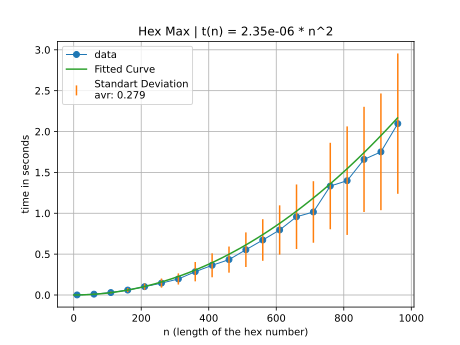
\includegraphics[width=\textwidth]{Laufzeit.png}

Wie man sieht, passt diese angeglichene Funktion ziemlich gut. Der Funktionstherm wäre mit meinen Specs ca. $f(n) = 2.08e-06 \cdot 4^n$





\section{Umsetzung}

\subsection{Das generieren der Operanden}

In der Aufgabenstellung steht, dass die Aufgabe interessant sein muss. Dies impliziert 2 Sachen:

\begin{enumerate}
\item Die Operanden müssen divers sein,
\item Die Operatoren müssen divers sein.
\end{enumerate}

Jetzt ist normaler 'Zufall' nicht divers oder spannend genug, da sich gleiche Zahlen häufen können. Dies will ich nicht, daher erstelle ich eine Art Zwischenspeicher\footnote{lediglich eine Liste}, in dem alle noch nicht genutzten Zahlen vorhanden sind. Dann mische ich diesen und lasse eine Iteration eines Sortieralgorithmusses drüber laufen. Dies mache ich damit es warscheinlicher ist, dass große Zahlen vor Kleinen kommen. Dies erhöht die Warscheinlichkeit auf eine mögliche Division\footnote{da immer ganze Zahlen Zwischenergebnis sein müssen} um einiges.

Das oben Beschriebene war das Auffüllen des Zwischenspeichers. Er wird immer dann aufgefüllt, wenn er leer ist. Anschließend fülle ich die Liste an Operanden auf. Das heißt, ich nehme immer das erste Element des Zwischenspeichers, füge es zu den Operanden hinzu und entferne es aus dem Zwischenspeicher. Dies mache ich jedes mal, außer der zuletzt hinzugefügte Operand ist mit einem beliebigen Element aus dem Zwischenspeicher teilbar. Dann füge ich dieses Element aus dem Zwischenspeicher hinzu. Somit habe ich genug Chancen auf eine Division.

Das alles mache ich so lange, bis ich eine Liste mit $n$ Operanden habe.

\newpage
\subsection{Alle möglichen Operatoren ausprobieren}

Es gibt 4 Operatoren.

\begin{enumerate}
\item $+$
\item $-$
\item $\cdot$
\item $/$
\end{enumerate}

Da ich jede mögliche Operatorenkombination für $n$ Operanden ausprobieren muss, lässt mich das mit $4^{n}$ Iterationen zurück. Das heißt, ich starte eine for-Schleife, die $4^{n}$ Iterationen durchläuft. Vorher initialisiere ich jedoch ein dictionary, bei dem der key das resultierende Ergebnis ist. Dies ermöglicht mir schnelles Auslesen. Der Wert hinter dem Key besteht aus 3 weiteren Werten. Der Frequenz, dem Therm und nochmals dem Ergebnis\footnote{Hätte ich es später implementiert, hätte ich das Ergebnis wegen des Arbeitsspeichers weggelassen}. Auch initialisiere ich eine Liste der Länge $n$, bei der alle Element 0 sind. Jedes Element dieser Liste repräsentiert einen Operator. + ist 0, - ist 1, * ist 2 und / ist 3.

Nach jeder Iteration erhöhe ich die Operatoren-Liste um 1. Dafür erhöhe ich zuerst das letzte Element. Ist es größer als 3, setzte ich es auf 0 und mache das gleiche mit dem vorherigen Element. Im Endeffekt ist das das gleiche, wie in base-4 zu zählen.

Am Anfang der Schleife wandle ich das ganze noch in einen 'Therm-String' um. Das bedeutet, ich wandle die Operanden in einen string um und schreibe die string-Repräsentation zwischen jede Ziffer\footnote{das Program macht das nicht genau so, aber ich sollte nicht auf jedes if-Statement eingehen}. Dieser kann dann beispielsweise so aussehen: '9 + 3 * 0'. Wenn ich ein solchen Therm habe, kann ich diesen effizient mit der in Python eingebauten \href{https://www.w3schools.com/python/ref_func_eval.asp}{eval()}-Funktion berechnen. Es ist aber bei diesem Vorgehen möglich, dass eine Division dabei ist, deren Zwischenergebnis keine ganze Zahl ist. Deshalb prüfe bei der Umwandlung in einen Therm-String jede Division mit modulo, ob diese illegal ist. Ist sie illegal, gehe ich einfach zur nächsten.

Mit dem berechneten Ergebnis schaue ich in dem vorher initialisierten dicitonary nach, ob das Ergebnis schon gespeichert wurde. Ist dies der Fall, dann setze ich 'frequency' bei diesem Ergebnis auf 2 und lösche den schon gespeicherten Therm \footnote{frequency lösche ich nicht, sodass das Ergebnis noch gespeichert ist}. Ich lösche diesen Therm anstatt den neuen zu speichern, da mein Arbeitsspeicher limitiert ist und es unnötig ist nicht zu tun. Ist das Ergebnis aber noch nicht in dem dicitionary, dann speichere ich den Therm, das Ergebnis und die frequency(1) unter dem Ergebnis im dictionary.
\\
\\
\paragraph{Das Zusammenführen und Auswählen des Therms}

Ist dies alles gemacht, kann ich einfach alle Ergebnisse und Therme mit einer 'frequency' von 1 herausschreiben, und sie nach der Häufigkeit der Divisionen sortieren. Dies macht Sinn, da ich aufgrund der strikten Einschränkungen von Divisionen meist weniger diese Operatoren habe und das somit die Diversität verringert. Hab ich die Therme sortiert, kann ich einfach den Besten nehmen und habe ggf. noch mehr Aufgaben mit den gleichen Operanden. Es ist auch möglich, dass es mit diesen Operanden keinen einzigen validen Therm gibt. Dann generiere ich noch eimal neue Operanden und wiederhole alle. Die Warscheinlichkeit dafür ist nicht sonderlich hoch.

\subsection{multiprocessing}

Für alle Aufgaben mit $n < 8$ mach ich das oben Beschriebene, sonst lohnt es sich multiprocessing zu nutzen.

Diese Aufgabe zu parallelisieren war einfach. Das einzige was man machen musste war, $x$ Threads zu starten\footnote{4 bei mir, da ich 4 cores habe} und statt in einem Thread $4^n$ Iterationen zu machen, in jedem Thread $\frac{4^n}{x}$ Iterationen zu machen und die Startzahl entsprechend zu wählen. Da ich 4 Threads verwendet habe, war das Zusammenführen weniger das Problem, weil es kaum Überschneidungen in den Ergebnissen gibt. Das kommt daher, dass ich 4 Operatoren habe und in jedem Thread einer überwiegt. Das führt leider auch dazu, dass der Thread der die ganzen Divisionen durführt, etwas länger braucht.


\section{Erweiterung}

Meine Methode der Validierung und des Findens der Therme ermöglicht mir, eine Aufgabe für die meisten Operanden die man selber definieren kann zu generieren. Also habe ich dies implementiert und ein Konsolenprogramm gemacht. Wenn Sie 'rechenrätsel.py' ausführen, können Sie 'n: <n>' eingeben um eine zufällige Zahlenfolge zu bekommen, oder Sie können die Operanden einfach mit einem Leerzeichen seperiert dort eingeben um eine Aufgabe mit diesen zu bekommen.

\subsection{Beispiele}

Hier habe ich dies mit ein paar lustigen und tollen Zahlenfolgen gemacht.

\paragraph{PI}

3 1 4 1 5 9 2 6 5 3 5 8\\
3 ◦ 1 ◦ 4 ◦ 1 ◦ 5 ◦ 9 ◦ 2 ◦ 6 ◦ 5 ◦ 3 ◦ 5 ◦ 8 = 783\\
3 - 1 - 4 - 1 - 5 - 9 + 2 * 6 * 5 / 3 * 5 * 8 = 783

\paragraph{Fibonacci}

1 1 2 3 5 8\\
0 ◦ 7 ◦ 6 ◦ 2 ◦ 5 ◦ 3 = 102\\
0 + 7 * 6 / 2 * 5 - 3 = 102

\paragraph{69}

6 9\\
6 ◦ 9 = 15\\
6 + 9 = 15

\paragraph{range}

0 1 2 3 4 5 6 7 8 9\\
0 + 1 - 2 + 3 * 4 * 5 / 6 * 7 * 8 - 9 = 550\\
0 ◦ 1 ◦ 2 ◦ 3 ◦ 4 ◦ 5 ◦ 6 ◦ 7 ◦ 8 ◦ 9 = 550

\section{Beispiele}

Hier sind für $0 \leq n \leq 15$ jeweils 3 Beispiele. Wollen Sie mehr oder andere, dann schauen Sie in solutions/exampels.txt.

Das Format in dem ich die Beispiele aufschreibe ist:
\\
\\
<Aufgabe>\\
<Lösung>\\
<Dauer der Ausführung>\\
\\
<Aufgabe>\\
<Lösung>\\
<Dauer der Ausführung>\\

\noindent und immer so weiter.

\paragraph{$n=0$} \hrulefill
\\
\\
Hier ist ein Edge case. In meinem Programm frage ich, ob $n=0$ und wenn das so ist, dann gibt es eine zufällige Zahl von 0-9 zurück. Daher gebe ich hier nur ein Beispiel, da es uninteressant ist.
\\
\\
7 = 7\\
7 = 7\\
0.00 Sekunden\\
\paragraph{$n=1$} \hrulefill
\\
\\
2 ◦ 4 = 6\\
2 + 4 = 6\\
0.00 Sekunden\\
\\
7 ◦ 9 = 63\\
7 * 9 = 63\\
0.00 Sekunden\\
\\
5 ◦ 3 = 2\\
5 - 3 = 2\\
0.00 Sekunden\\
\paragraph{$n=2$} \hrulefill
\\
\\
9 ◦ 3 ◦ 0 = 9\\
9 + 3 * 0 = 9\\
0.00 Sekunden\\
\\
9 ◦ 2 ◦ 0 = 9\\
9 + 2 * 0 = 9\\
0.00 Sekunden\\
\\
9 ◦ 6 ◦ 2 = 12\\
9 + 6 / 2 = 12\\
0.00 Sekunden\\
\paragraph{$n=3$} \hrulefill
\\
\\
7 ◦ 6 ◦ 3 ◦ 1 = 8\\
7 + 6 / 3 - 1 = 8\\
0.00 Sekunden\\
\\
3 ◦ 5 ◦ 0 ◦ 9 = 12\\
3 + 5 * 0 + 9 = 12\\
0.00 Sekunden\\
\\
2 ◦ 3 ◦ 4 ◦ 1 = 13\\
2 + 3 * 4 - 1 = 13\\
0.00 Sekunden\\
\paragraph{$n=4$} \hrulefill
\\
\\
5 ◦ 4 ◦ 2 ◦ 6 ◦ 3 = 38\\
5 * 4 * 2 - 6 / 3 = 38\\
0.01 Sekunden\\
\\
6 ◦ 2 ◦ 8 ◦ 4 ◦ 1 = 34\\
6 / 2 + 8 * 4 - 1 = 34\\
0.00 Sekunden\\
\\
5 ◦ 2 ◦ 1 ◦ 9 ◦ 3 = 7\\
5 - 2 + 1 + 9 / 3 = 7\\
0.00 Sekunden\\
\paragraph{$n=5$} \hrulefill
\\
\\
7 ◦ 8 ◦ 2 ◦ 6 ◦ 3 ◦ 9 = 156\\
7 * 8 / 2 * 6 - 3 - 9 = 156\\
0.01 Sekunden\\
\\
5 ◦ 7 ◦ 1 ◦ 2 ◦ 8 ◦ 4 = 35\\
5 * 7 + 1 * 2 - 8 / 4 = 35\\
0.01 Sekunden\\
\\
9 ◦ 3 ◦ 6 ◦ 2 ◦ 1 ◦ 5 = 75\\
9 * 3 * 6 / 2 - 1 - 5 = 75\\
0.01 Sekunden\\
\paragraph{$n=6$} \hrulefill
\\
\\
3 ◦ 0 ◦ 8 ◦ 4 ◦ 2 ◦ 5 ◦ 7 = 78\\
3 * 0 + 8 + 4 / 2 * 5 * 7 = 78\\
0.03 Sekunden\\
\\
8 ◦ 4 ◦ 2 ◦ 3 ◦ 1 ◦ 5 ◦ 7 = 82\\
8 * 4 / 2 * 3 - 1 + 5 * 7 = 82\\
0.16 Sekunden\\
\\
9 ◦ 3 ◦ 6 ◦ 2 ◦ 4 ◦ 7 ◦ 1 = 316\\
9 * 3 * 6 / 2 * 4 - 7 - 1 = 316\\
0.06 Sekunden\\
\paragraph{$n=7$} \hrulefill
\\
\\
1 ◦ 6 ◦ 3 ◦ 7 ◦ 4 ◦ 2 ◦ 5 ◦ 8 = 240\\
1 + 6 * 3 * 7 * 4 / 2 - 5 - 8 = 240\\
0.23 Sekunden\\
\\
9 ◦ 3 ◦ 5 ◦ 8 ◦ 2 ◦ 4 ◦ 7 ◦ 0 = 529\\
9 * 3 * 5 * 8 / 2 - 4 - 7 + 0 = 529\\
0.13 Sekunden\\
\\
0 ◦ 9 ◦ 3 ◦ 8 ◦ 4 ◦ 2 ◦ 6 ◦ 5 = 421\\
0 + 9 * 3 * 8 * 4 / 2 - 6 - 5 = 421\\
0.43 Sekunden\\
\paragraph{$n=8$} \hrulefill
\\
\\
7 ◦ 3 ◦ 1 ◦ 0 ◦ 8 ◦ 4 ◦ 2 ◦ 9 ◦ 6 = 143\\
7 - 3 + 1 + 0 + 8 * 4 / 2 * 9 - 6 = 143\\
0.72 Sekunden\\
\\
2 ◦ 0 ◦ 5 ◦ 3 ◦ 8 ◦ 4 ◦ 6 ◦ 7 ◦ 1 = 246\\
2 * 0 - 5 + 3 * 8 / 4 * 6 * 7 - 1 = 246\\
0.71 Sekunden\\
\\
6 ◦ 2 ◦ 1 ◦ 7 ◦ 8 ◦ 4 ◦ 9 ◦ 3 ◦ 0 = 214\\
6 / 2 - 1 + 7 * 8 * 4 - 9 - 3 + 0 = 214\\
0.73 Sekunden\\
\paragraph{$n=9$} \hrulefill
\\
\\
0 ◦ 7 ◦ 6 ◦ 5 ◦ 8 ◦ 2 ◦ 3 ◦ 9 ◦ 1 ◦ 4 = 313\\
0 + 7 * 6 * 5 + 8 / 2 * 3 * 9 - 1 - 4 = 313\\
0.98 Sekunden\\
\\
8 ◦ 2 ◦ 5 ◦ 9 ◦ 3 ◦ 0 ◦ 4 ◦ 6 ◦ 7 ◦ 1 = 524\\
8 / 2 * 5 * 9 * 3 + 0 - 4 - 6 - 7 + 1 = 524\\
0.99 Sekunden\\
\\
0 ◦ 9 ◦ 6 ◦ 2 ◦ 5 ◦ 7 ◦ 8 ◦ 4 ◦ 3 ◦ 1 = 823\\
0 - 9 + 6 / 2 * 5 * 7 * 8 - 4 - 3 - 1 = 823\\
0.95 Sekunden\\
\paragraph{$n=10$} \hrulefill
\\
\\
6 ◦ 2 ◦ 4 ◦ 3 ◦ 7 ◦ 5 ◦ 9 ◦ 0 ◦ 8 ◦ 4 ◦ 1 = 227\\
6 / 2 * 4 * 3 * 7 - 5 - 9 + 0 - 8 - 4 + 1 = 227\\
2.19 Sekunden\\
\\
0 ◦ 7 ◦ 9 ◦ 9 ◦ 6 ◦ 2 ◦ 4 ◦ 5 ◦ 1 ◦ 8 ◦ 3 = 452\\
0 - 7 - 9 - 9 + 6 / 2 * 4 * 5 * 1 * 8 - 3 = 452\\
2.95 Sekunden\\
\\
8 ◦ 2 ◦ 9 ◦ 3 ◦ 5 ◦ 7 ◦ 1 ◦ 4 ◦ 0 ◦ 6 ◦ 6 = 1663\\
8 * 2 * 9 / 3 * 5 * 7 - 1 - 4 + 0 - 6 - 6 = 1663\\
2.44 Sekunden\\
\paragraph{$n=11$} \hrulefill
\\
\\
0 ◦ 8 ◦ 2 ◦ 5 ◦ 3 ◦ 2 ◦ 7 ◦ 9 ◦ 4 ◦ 1 ◦ 8 ◦ 6 = 1834\\
0 - 8 / 2 + 5 * 3 * 2 * 7 * 9 - 4 - 1 * 8 * 6 = 1834\\
5.86 Sekunden\\
\\
4 ◦ 2 ◦ 6 ◦ 3 ◦ 1 ◦ 9 ◦ 8 ◦ 5 ◦ 0 ◦ 7 ◦ 7 ◦ 6 = 1140\\
4 * 2 * 6 / 3 * 1 * 9 * 8 - 5 + 0 - 7 / 7 - 6 = 1140\\
7.52 Sekunden\\
\\
1 ◦ 0 ◦ 9 ◦ 3 ◦ 2 ◦ 4 ◦ 6 ◦ 5 ◦ 8 ◦ 7 ◦ 7 ◦ 3 = 1252\\
1 * 0 + 9 * 3 * 2 * 4 * 6 - 5 * 8 - 7 / 7 - 3 = 1252\\
7.39 Sekunden\\
\paragraph{$n=12$} \hrulefill
\\
\\
2 ◦ 1 ◦ 7 ◦ 4 ◦ 5 ◦ 3 ◦ 9 ◦ 8 ◦ 0 ◦ 6 ◦ 6 ◦ 2 ◦ 4 = 998\\
2 - 1 - 7 - 4 + 5 * 3 * 9 * 8 + 0 - 6 * 6 / 2 * 4 = 998\\
22.32 Sekunden\\
\\
7 ◦ 4 ◦ 9 ◦ 3 ◦ 1 ◦ 4 ◦ 0 ◦ 6 ◦ 3 ◦ 1 ◦ 8 ◦ 2 ◦ 5 = 672\\
7 * 4 * 9 * 3 - 1 - 4 + 0 + 6 / 3 - 1 - 8 * 2 * 5 = 672\\
31.39 Sekunden\\
\\
0 ◦ 5 ◦ 5 ◦ 8 ◦ 4 ◦ 7 ◦ 8 ◦ 2 ◦ 1 ◦ 6 ◦ 3 ◦ 4 ◦ 9 = 426\\
0 - 5 - 5 - 8 * 4 + 7 * 8 / 2 * 1 * 6 * 3 - 4 * 9 = 426\\
36.33 Sekunden\\
\paragraph{$n=13$} \hrulefill
\\
\\
4 ◦ 2 ◦ 5 ◦ 0 ◦ 6 ◦ 3 ◦ 8 ◦ 1 ◦ 9 ◦ 7 ◦ 7 ◦ 5 ◦ 9 ◦ 3 = 7033\\
4 - 2 * 5 + 0 + 6 / 3 * 8 * 1 * 9 * 7 * 7 - 5 - 9 - 3 = 7033\\
105.48 Sekunden\\
\\
3 ◦ 5 ◦ 1 ◦ 2 ◦ 4 ◦ 7 ◦ 6 ◦ 9 ◦ 8 ◦ 0 ◦ 7 ◦ 6 ◦ 3 ◦ 8 = 1228\\
3 * 5 * 1 * 2 * 4 * 7 / 6 * 9 - 8 + 0 - 7 - 6 - 3 - 8 = 1228\\
83.34 Sekunden\\
\\
9 ◦ 5 ◦ 6 ◦ 7 ◦ 8 ◦ 2 ◦ 5 ◦ 7 ◦ 8 ◦ 3 ◦ 0 ◦ 4 ◦ 2 ◦ 1 = 1490\\
9 * 5 * 6 * 7 * 8 / 2 / 5 - 7 - 8 + 3 * 0 - 4 - 2 - 1 = 1490\\
111.23 Sekunden\\
\paragraph{$n=14$} \hrulefill
\\
\\
3 ◦ 4 ◦ 2 ◦ 8 ◦ 9 ◦ 9 ◦ 3 ◦ 2 ◦ 7 ◦ 4 ◦ 1 ◦ 0 ◦ 5 ◦ 7 ◦ 6 = 40802\\
3 * 4 / 2 * 8 * 9 * 9 * 3 / 2 * 7 - 4 + 1 * 0 - 5 - 7 - 6 = 40802\\
452.86 Sekunden\\
\\
0 ◦ 5 ◦ 1 ◦ 6 ◦ 3 ◦ 4 ◦ 7 ◦ 9 ◦ 9 ◦ 3 ◦ 4 ◦ 2 ◦ 0 ◦ 8 ◦ 2 = 15307\\
0 - 5 - 1 + 6 * 3 * 4 * 7 * 9 * 9 * 3 / 4 / 2 + 0 + 8 / 2 = 15307\\
468.41 Sekunden\\
\\
9 ◦ 3 ◦ 7 ◦ 8 ◦ 2 ◦ 1 ◦ 6 ◦ 5 ◦ 4 ◦ 2 ◦ 8 ◦ 4 ◦ 3 ◦ 5 ◦ 0 = 4741\\
9 - 3 - 7 * 8 - 2 - 1 - 6 + 5 * 4 / 2 * 8 * 4 * 3 * 5 + 0 = 4741\\
402.92 Sekunden\\
\paragraph{$n=15$} \hrulefill
\\
\\
5 ◦ 3 ◦ 9 ◦ 8 ◦ 8 ◦ 2 ◦ 9 ◦ 3 ◦ 6 ◦ 5 ◦ 7 ◦ 0 ◦ 6 ◦ 2 ◦ 1 ◦ 4 = 38834\\
5 * 3 * 9 * 8 * 8 / 2 * 9 - 3 - 6 * 5 + 7 * 0 - 6 - 2 - 1 - 4 = 38834\\
1870.65 Sekunden\\
\\
7 ◦ 9 ◦ 3 ◦ 2 ◦ 6 ◦ 1 ◦ 0 ◦ 5 ◦ 2 ◦ 6 ◦ 3 ◦ 4 ◦ 8 ◦ 1 ◦ 5 ◦ 0 = 1392\\
7 * 9 / 3 * 2 * 6 - 1 + 0 - 5 + 2 * 6 * 3 * 4 * 8 - 1 - 5 + 0 = 1392\\
2502.59 Sekunden\\
\\
4 ◦ 2 ◦ 8 ◦ 6 ◦ 6 ◦ 3 ◦ 5 ◦ 4 ◦ 2 ◦ 1 ◦ 7 ◦ 9 ◦ 3 ◦ 0 ◦ 5 ◦ 1 = 15346\\
4 * 2 * 8 * 6 * 6 / 3 * 5 * 4 - 2 - 1 + 7 - 9 - 3 + 0 - 5 - 1 = 15346\\
2258.38 Sekunden\\



\section{Quellcode}

\lstset{
	language=python, 				% Setzt die Sprache
}
\begin{lstlisting}
from multiprocessing import Pool, freeze_support
import random


def generate_operands(n, minimum=0, maximum=9):
    """
    generiert eine Liste von Operanden der Laenge n

    :param n: die Anzahl an Operatoren
    :param minimum: der kleinst moegliche Operand
    :param maximum: der groesstmoegliche Operand
    :return: liste von Operanden der Laenge n
    """
    # liste aller Operanden
    operands = []
    # queue fuer die Operanden, da 'echter' Zufall langweilig ist
    unused_operands = []

    # auffuellen der queue
    def refresh_unused_operands():
        nonlocal unused_operands
        unused_operands = list(range(minimum, maximum + 1))
        random.shuffle(unused_operands)
        for i, unused_operator in enumerate(unused_operands):
            if random.randint(0, 1) == 0:
                index_difference = random.randint(1, 2)
                if i - index_difference >= 0:
                    if i - index_difference > unused_operator:
                        unused_operands[i] = unused_operands[i - index_difference]
                        unused_operands[i - index_difference] = unused_operator

    refresh_unused_operands()

    # generiere Liste von Operanden mit der queue
    new_operand = None
    for i in range(n + 1):
        if len(operands) != 0:
            last_operand = operands[-1]
            # wenn der letzte Operand durch einen der noch in der queue ist teilbar ist, nehme diesen
            for i, unused_operand in enumerate(unused_operands):
                if unused_operand != 0 and unused_operand != 1:
                    if last_operand % unused_operand == 0:
                        new_operand = unused_operand
                        unused_operands.pop(i)
                        break

        if new_operand is None:
            new_operand = unused_operands[0]
            unused_operands.pop(0)

        if len(unused_operands) == 0:
            refresh_unused_operands()

        operands.append(new_operand)
        new_operand = None

    return operands


def maybe_get_therm(n, operands, minimum=0, maximum=9):
    """
        generiert eine Liste von Operanden
        sucht alle eindeutigen Therme
        gibt alle eindeutigen Therme zurueck

        :param n: die Anzahl an Operatoren
        :param operands: optional zu n einfach die Operanden
        :param minimum: der kleinstmoegliche Operand
        :param maximum: der groesstmoegliche Operand
        :return: Liste potenzieller Loesungen
    """

    OPERATORS = [" + ", " - ", " * ", " / "]

    # generiere ein liste von Operanden oder nimmt die uebergebene
    if operands is None:
        operands = generate_operands(n=n, minimum=minimum, maximum=maximum)

    result_frequencies = compute_combinations(part=0, n=n, operands=operands, threads=1)

    unique_therms = []
    for key in result_frequencies:
        if result_frequencies[key]["freq"] == 1:
            unique_therms.append({
                'therm': result_frequencies[key]['therm'],
                'result': result_frequencies[key]['result']
            })

    return unique_therms


def compute_combinations(part, n, operands, threads=4):
    OPERATORS = [
        " + ",
        " - ",
        " * ",
        " / "
    ]

    def get_real_therm(operands_, operators_):
        therm_string = str(operands_[0])

        multiplication_sub = 1
        for i, operator_ in enumerate(operators_):
            if operator_ == 2:
                multiplication_sub = multiplication_sub * operands_[i]
            elif operator_ == 3:
                if operands_[i + 1] == 0 or multiplication_sub * operands_[i] / operands_[i + 1] % 1 != 0:
                    return ""
            elif operator_ == 0 or operator_ == 1:
                multiplication_sub = 1
            therm_string += OPERATORS[operator_]
            therm_string += str(operands_[i + 1])
        return therm_string

    result_frequencies = {

    }

    last_list = [0] * n
    last_list[0] = part
    last_list[-1] = -1

    for i in range(int((4 ** n) / threads)):
        for i, elem in enumerate(reversed(last_list)):
            i = len(last_list) - i - 1
            if elem > 2:
                last_list[i] = 0
            else:
                last_list[i] += 1
                break

        therm = get_real_therm(operands, last_list)
        if therm != "":
            result = eval(therm)
            if result <= 0:
                continue
            if result % 1 != 0:
                continue

            if result in result_frequencies:
                result_frequencies[result]['freq'] += 1
            else:
                result_frequencies[result] = {'freq': 1, 'therm': therm, 'result': int(result)}

    return result_frequencies


def maybe_get_therm_multiprocessing(n, operands, minimum=0, maximum=9):
    """
    generiert eine Liste von Operanden
    started threads, die jeweils ein Teil aller Loesungen eindeutigen Therme
    schaut wenn alle threads fertig sind ob die Loesungen wirklich eindeutig sind,
    gibt alle eindeutigen Therme zurueck

    :param n: die Anzahl an Operatoren
    :param operands: optional zu n einfach die Operanden
    :param minimum: der kleinst moegliche Operand
    :param maximum: der groesstmoegliche Operand
    :return: liste potenzieller Loesungen
    """

    # generiere ein liste von operanden oder nimmt die uebergebene
    if operands is None:
        operands = generate_operands(n=n, minimum=minimum, maximum=maximum)

    with Pool() as pool:
        result = pool.starmap(compute_combinations,
                              [(0, n, operands), (1, n, operands), (2, n, operands), (3, n, operands)])
        print("multiprocessing done")

        unique_therms = []

        for i in range(len(result)):
            for key in result[i]:
                is_unique = True
                for j in range(len(result)):
                    if j == i:
                        continue
                    if key in result[j]:
                        is_unique = False
                        result[j].pop(key)
                if is_unique:
                    unique_therms.append({
                        'therm': result[i][key]['therm'],
                        'result': key
                    })

        return unique_therms


def get_therm(n: int, operands: list=None, minimum=0, maximum=9):
    """
    https://bwinf.de/fileadmin/bundeswettbewerb/40/aufgaben402.pdf
    Diese Funktion loest die Aufgabe Rechenraetsel

    :param n: die Anzahl an Operatoren
    :param operands: optional zu n einfach die Operanden
    :param minimum: der kleinstmoegliche Operand
    :param maximum: der groesstmoegliche Operand
    :return: tuple (Loesung, Aufgabe)
    """

    # edge cases
    if n < 0:
        return "No.", "still No."
    if n == 0:
        random_number = random.randint(minimum + 1, maximum)
        return f"{random_number} = {random_number}", f"{random_number} = {random_number}"

    mixing_afterwards = True
    if operands is not None:
        mixing_afterwards = False

    """
    fuellt die Liste mit moeglichen Ergebnissen auf.
    nutzt ab n < 8 Parallelisierung, da vorher thread pulling 
    laenger als die eigentliche Aufgabe braucht.
    """
    results = []
    while not len(results):
        if n < 8:
            results = maybe_get_therm(n, operands, minimum=minimum, maximum=maximum)
        else:
            results = maybe_get_therm_multiprocessing(n, operands, minimum=minimum, maximum=maximum)
        operands = None

    """
    da negative operatoren (-, /) vergleichsweise selten sind suche die Loesung
    mit der hoechsten Anzahl von diesen heraus
    """

    def negative_operators(result_: dict):
        therm_str = result_['therm']
        if not therm_str.count('/'):
            return 0
        return therm_str.count('-') + therm_str.count('/')

    best_result = results[random.randrange(len(results))]
    best_diversity = 0
    for result in results:
        diversity = negative_operators(result)
        if diversity > best_diversity:
            best_diversity = diversity
            best_result = result

    if best_diversity == 0 and n > 3:
        # wenn es mehr als 3 Operatoren gibt muss mindestens ein negativer Operator
        # enthalten sein
        return get_therm(n, minimum=minimum, maximum=maximum)

    print(f"best operator diversity: {best_diversity}")

    result = best_result['result']
    therm = best_result['therm']

    # mische den Therm noch einmal
    def mix_therm():
        therm_list = therm.split(" + ")
        random.shuffle(therm_list)
        return " + ".join(therm_list)

    # entferne die operatoren
    def censor_therm(therm_: str):
        return therm_.replace(" + ", u" o ").replace(" - ", u" o ").replace(" * ", u" o ").replace(" / ", u" o ")

    if mixing_afterwards:
        finished_therm = mix_therm()
    else:
        finished_therm = therm

    return f"{finished_therm} = {int(result)}", f"{censor_therm(finished_therm)} = {int(result)}"


if __name__ == "__main__":
    freeze_support()
    while True:
        input_ = input("\ntype 'n: <n>' to specify n else just type the desired operands seperated by space: ")
        if input_ == "exit":
            break

        if "n:" in input_:
            n = int(input_.split(":")[1])
            operands = None
        else:
            try:
                operands = [int(x) for x in input_.split(" ")]
                n = len(operands) - 1
            except ValueError:
                print("invalid input")
                continue

        print("computing...")
        print(get_therm(n, operands=operands))


\end{lstlisting}

\end{document}
